\section{Motivation \& Background}


\begin{frame}[t]{The probability distribution revolution}
	\begin{multicols}{2}
		\begin{itemize}
			\item Karl Pearson (1857-1936) came with the idea that scientific measurements should be conceived as coming from probability distributions.
			\item Scientific measurements are just random reflections of the underlying truth that is the distribution.
			\item “A great book on the
history of statistics” $\rightarrow$ Aaron
			\item
		\end{itemize}

		\columnbreak

		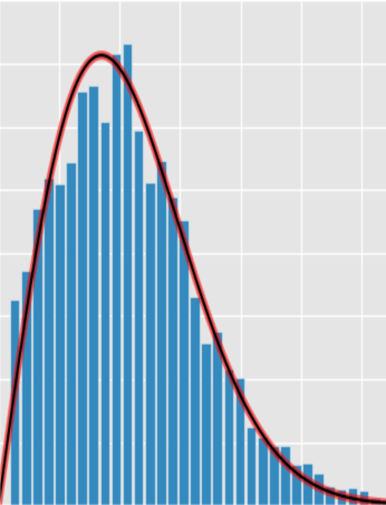
\includegraphics[width=0.25\textwidth]{media/distribution}
		\linebreak
		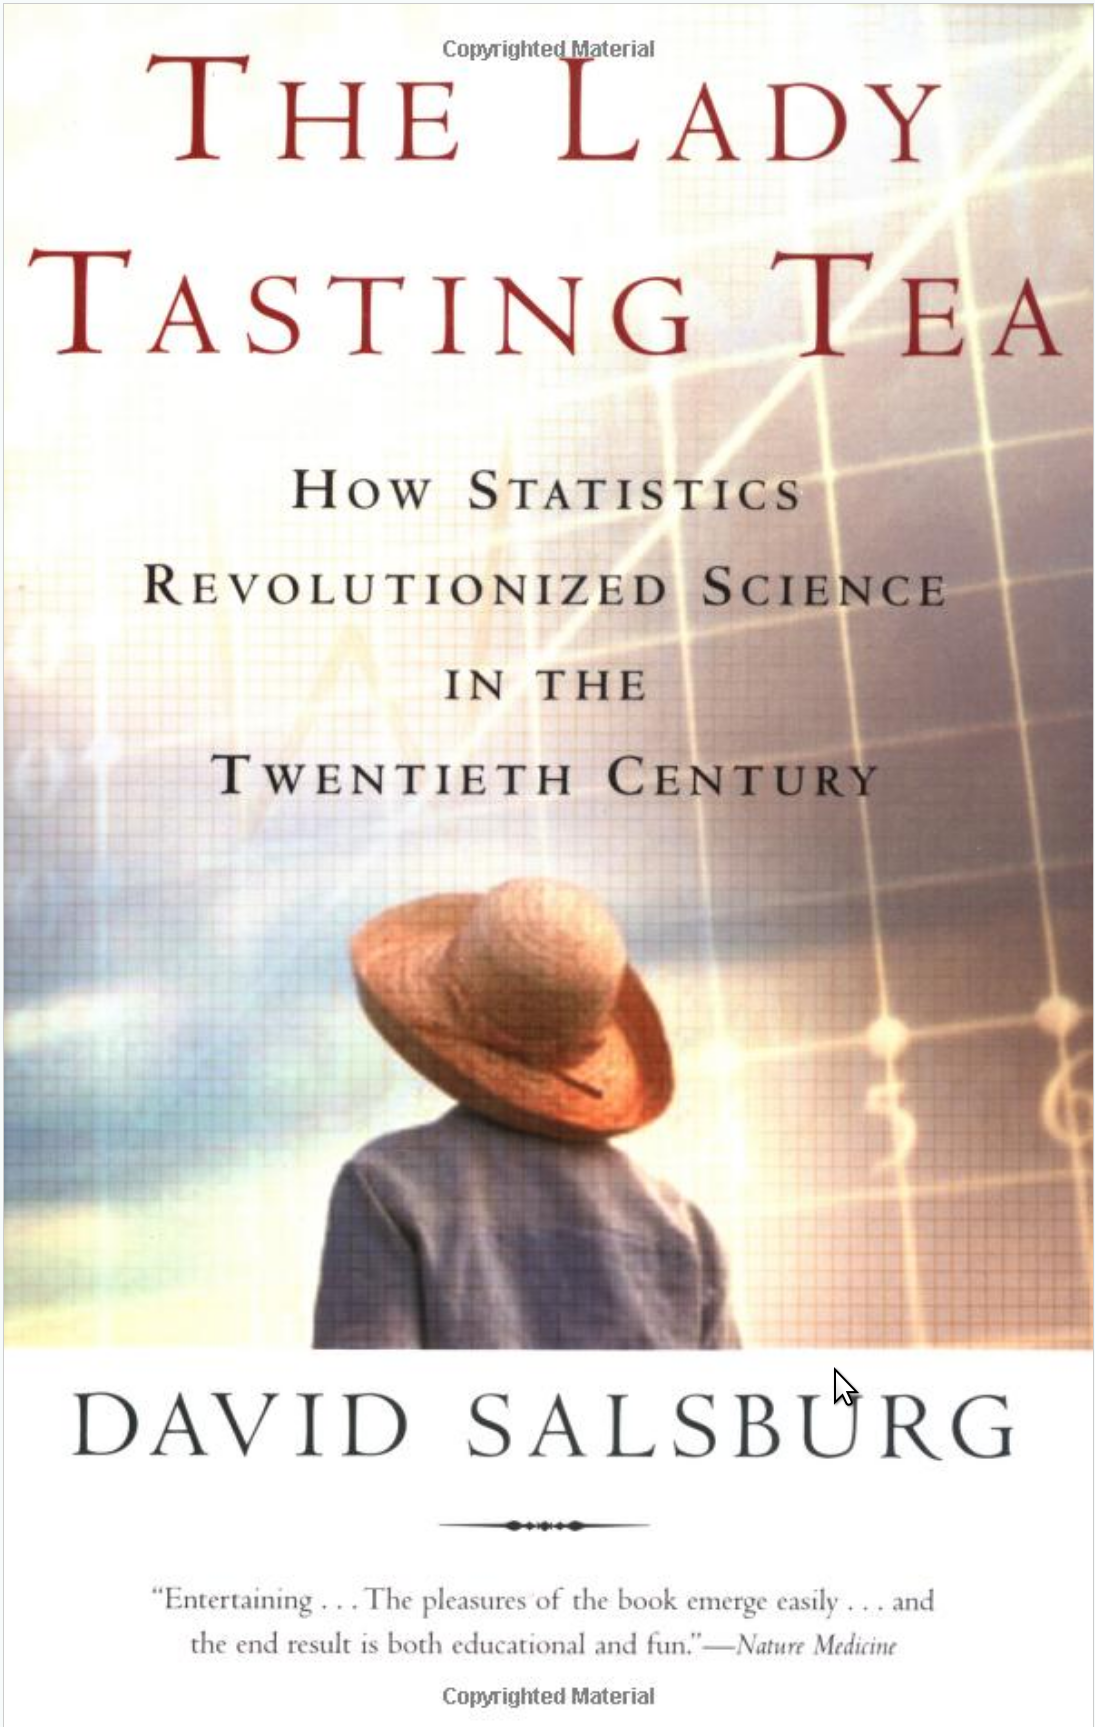
\includegraphics[width=0.25\textwidth]{media/book}
	\end{multicols}

	\note{Lets start with a bit of history. The idea that scientific measurements are best understood as reflecting underlying probabilities distributions is a relatively new idea.

It was a now famous thinker and scientist, Karl Pearson (of the Pearson correlation coefficient) who conceived the idea in late 18 hundreds.

He realized randomness was inherent part of nature and of scientific measure, and he formulated the idea that all measurments should be conceived of as coming from an underlying probability distributions.

In other words, the underlying truth is the distrubutions, and the measurements are just random reflections of this truth.  At the time, this was a revolutionary idea.}
\end{frame}

\begin{frame}[t]{The power of probability distributions}
	Distributions allow scientists to:
	\begin{itemize}
		\item Understand scientific measurement
		\item Predict the probability of specific data
		\item Test specific hypothesis (p-values)
		\item Produce generative models
		\item Better conceptual understanding data.
	\end{itemize}
	\note{And it was an idea that revolutized science.

	It allowed scientists to:
	\begin{itemize}
		\item Better understand their measurements.
		\item To make predictions about what data they should expect to observe.
		\item To test scientific hypotheses in a mathematically rigorous way.
		\item To build generative models of their data, and to test how well those models explain the observed measurments.
		\item And in general to have a better conceptual understanding of the data they generated.
	\end{itemize}
}
\end{frame}
%--- Next Frame ---%

\begin{frame}[t]{Estimating distributions from data}
	\begin{multicols}{2}
		Low-Dimensional:
		\begin{itemize}
			\item Great tools to fit and understand the underlying probability distribution of data.
		\end{itemize}
		\vfill\columnbreak
		High-Dimensional:
		\begin{itemize}
			\item In some cases, classical statistical tools are insufficient.
			\item Problematic for modern neuroscience: \begin{itemize}
				\item Thousands of electrodes.
				\item Millions of voxels.
			\end{itemize}
		\end{itemize}
	\end{multicols}
	\note{Since Pearson’s early work, scientists and statisticians have devised an enormous number of related tools.

For example they’ve defined many many distributions, and they’ve created tools for working with those distrubitons (calculating likelihoods and fitting them).

One class of tools aim to estimate the underlying distribution that generated an observed empirical measurment.

These tools are highly effective when data is low dimensional, but they are sometimes insufficient when data is high dimensional.}
\end{frame}
%--- Next Frame ---%

\begin{frame}[t]{How can we build statistical distributions for neuroscience datasets?}
	\movie[]{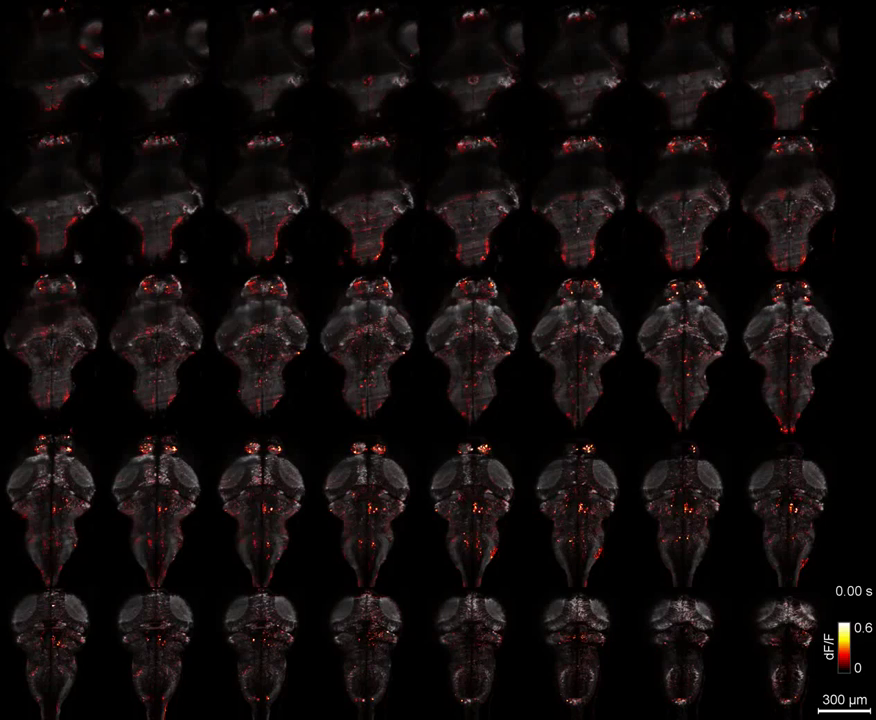
\includegraphics[width=0.7\textwidth,center]{media/zfish_first.png}}{media/zfish_imaging.mp4}
	\nakedfootnote{\url{https://www.youtube.com/watch?v=CXYp9xCUhe0}}
	\note{For example, consider whole brain imaging data from the zebrafish.  This data can have millions of dimensions, which makes estimating the understanding joint probability distribution difficult.  The number of possible states is enormous.  The voxels are not independent.  You can’t simply make a histogram or a heat-map.
			}
\end{frame}
